\documentclass[tikz,dvipsnames]{standalone}
\usetikzlibrary{backgrounds}
\usetikzlibrary{calc,positioning,shapes.misc}

\begin{document}
 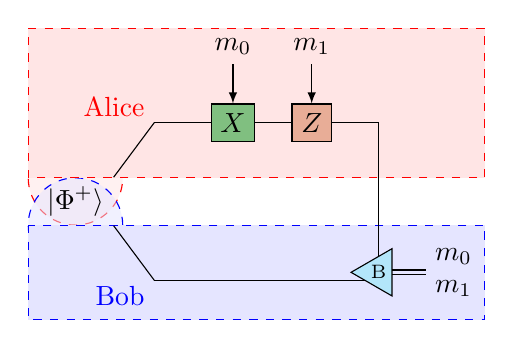
\begin{tikzpicture}[
    show background rectangle,
    tight background=0,
    background rectangle/.style={fill=white},
 ]
    \coordinate (A) at (0,+1.0);
    \coordinate (B) at (0,-1.0);
    \coordinate (E) at (-1,0);
    
    \draw[red,fill=Red!10,fill opacity=0.5,dashed,rounded corners=6pt] 
     ($(E)+(0,+0.3)$) circle (0.6);
    \draw[blue,fill=Blue!10,fill opacity=0.5,dashed,rounded corners=3pt] 
     ($(E)+(0,-0.3)$) circle (0.6);
    
    \draw[dashed,anchor=east,red,fill=red!10] 
    (E)++(-0.6,+0.3) rectangle (4.2,+2.2) (A)++(0,+0.2)
    node[opacity=1] {Alice};
    \draw[dashed,anchor=east,blue,fill=blue!10] 
    (E)++(-0.6,-0.3) rectangle (4.2,-1.5) (B)++(0,-0.2)
    node[opacity=1] {Bob};

    \node at (E) (EE) {$|\Phi^+\rangle$};
    \draw (EE.north east) -- (A);
    \draw (EE.south east) -- (B);
    \node[fill=Green!50   ,draw] at ($(A)+(1,0)$) (X)  {$X$};
    \node[fill=BrickRed!30,draw] at ($(A)+(2,0)$) (Z)  {$Z$};
    \node[above=0.5 of X] (M0) {$m_0$};
    \node[above=0.5 of Z] (M1) {$m_1$};
    \draw[-latex] (M0) -- (X); 
    \draw[-latex] (M1) -- (Z); 
    
    \coordinate (P) at ($(B)+(2.5,+0.1)$);
    \coordinate (Q) at ($(P)+(0.35,0)$);
    \draw (B) -- ($(Q)+(0,-0.1)$);

    \draw (A)--(X) -- (Z) -| ($(Q)+(0,+0.1)$);
     
    \draw (Q) ++(0,+0.03) -- ++(0.6,0) node[xshift=10pt,yshift=+5pt] {$m_0$};
    \draw (Q) ++(0,-0.03) -- ++(0.6,0) node[xshift=10pt,yshift=-5pt] {$m_1$};
    \filldraw[fill=cyan!30] (P) -- ++(30:0.6) -- ++(270:0.6) -- cycle;
    \node at (Q) {\scriptsize B};
\end{tikzpicture}
\end{document}
